\documentclass[12pt]{beamer}
\usetheme{Singapore}

\usepackage[utf8]{inputenc}
\usepackage[T1]{fontenc}
\usepackage{forest}
\usepackage{listings}

\author{Gianguido Sorà}

\title{Go in a nutshell}

\institute{Università degli Studi di Salerno}
	
\date{23/10/2015}

\titlegraphic{
\includegraphics[width=2cm]{/Users/gsora/Desktop/LDay2015/gologo.png}}


\setbeamercovered{transparent}
	
\setbeamertemplate{navigation symbols}{}

\begin{document}
	\maketitle
	
	% cos'è go
	\begin{frame}
		\frametitle{Cos'è Go}
		\begin{itemize}[<+->]
			\item Un linguaggio di programmazione
			\item Made in \textbf{Google}, sviluppato da \textbf{Robert Griesemer, Rob Pike, Ken Thompson}
			\item \textit{expressive, concise, clean and efficient}
		\end{itemize}
	\end{frame}
	
	% perché è cool
	\begin{frame}
		\frametitle{Perché è "cool"?}
		\begin{itemize}[<+->]
			\item compila in codice macchina
			\item è garbage-collected
			\item statically-typed, con reflection in run-time
			\item la sintassi è simile a quella di un linguaggio dinamico
			\item il modello di concorrenza integrato è facile da applicare
			\item è disponibile per tutti i maggiori OS...
			\item ...persino OpenBSD
			\item a partire dalla versione 1.4.1, il toolkit ed il compilatore sono completamente scritti in Go
		\end{itemize}
	\end{frame}
	
	%factorial
	\begin{frame}
		\begin{figure}
			\centering
			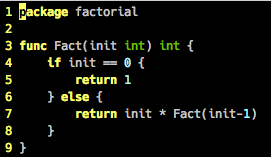
\includegraphics[width=0.7\linewidth]{factlib}
			\caption[Calcolo fattoriale]{Semplice libreria per il calcolo del fattoriale di un numero.}
			\label{fig:Schermata2015-10-23alle01}
		\end{figure}
	\end{frame}
	
	\begin{frame}
		\begin{figure}
			\centering
			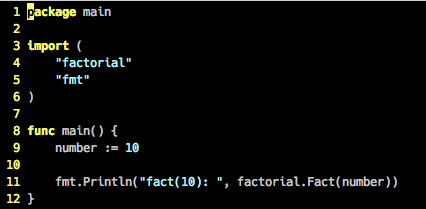
\includegraphics[width=0.7\linewidth]{factmain}
			\caption[Calcolo fattoriale]{Implementazione della libreria mostrata prima.}
			\label{fig:Schermata2015-10-23alle01}
		\end{figure}
	\end{frame}
	
	% il toolkit di go
	\begin{frame}
		\frametitle{Il toolkit di Go}
		\centering
		\begin{forest} mark/.style={circle}
			[Toolkit
				[comando "go"]
				[\$GOPATH]
			]
		\end{forest}
	\end{frame}
	
	% comando go
	\begin{frame}
		\frametitle{Il comando "go"}
		\begin{itemize}[<+->]
			\item  gestisce la compilazione e l'installazione di codice Go
			\item gestisce anche il testing...
			\item ...la documentazione dei pacchetti...
			\item ...le loro dipendenze (!)
			\item è simile ad un \textit{Makefile}, ma senza "make" e senza "configure"
			\item \textit{\$ go}
		\end{itemize}
	\end{frame}
	
	% il toolkit
	\begin{frame}
		\frametitle{Il toolkit}
		\begin{itemize}[<+->]
			\item Go è stato progettato per essere \textbf{developer-friendly}
			\item \textit{godoc} genera automaticamente la documentazione per pacchetto in base ai commenti scritti prima di ogni funzione, senza bisogno di particolare sintassi
			\item \textit{gofmt} formatta un sorgente Go dato in input secondo le guidelines di formattazione standard
			\item \url{https://golang.org/doc/cmd}
		\end{itemize}
	\end{frame}
	
	% $GOPATH
	\begin{frame}
		\frametitle{\textit{\$GOPATH}}
		\begin{itemize}[<+->]
			\item il codice Go deve essere tenuto in un \textbf{workspace}
			\item il workspace deve contenere le cartelle:
			\begin{itemize}
				\item \textit{src}: contiene i sorgenti organizzati in \textbf{pacchetti}
				\item \textit{pkg}: contiene i file oggetto generati, per ogni pacchetto
				\item \textit{bin}: eseguibili risultanti dalla compilazione
			\end{itemize}
			
			\item \textit{go build} compila un pacchetto contenuto in \textbf{src} e ne rende disponibile l'uso come libreria posando i file oggetto in \textbf{pkg}
			\item \textit{go install} compila un pacchetto che contiene un \textbf{main} e ne trasferisce il binario risultante in \textbf{bin}
			\item \textit{\$GOPATH} è il workspace su cui lavorare
			\item dev'essere settato a mano dallo sviluppatore
			\item è preferibile settare sia \textit{\$GOPATH} che \textit{\$GOPATH/bin} nella propria \textit{\$PATH}
		\end{itemize}
	\end{frame}
	
	% il sistema dei pacchetti
	\begin{frame}
		\frametitle{Il sistema dei pacchetti}
			\begin{itemize}[<+->]
				\item Go organizza il codice in unità chiamate \textbf{pacchetti}
				\item il pacchetto \textbf{"main"} è quello che contiene il metodo omonimo
				\item un pacchetto può avere un solo \textbf{main}
				\item un pacchetto può rappresentare una libreria
				\item i nomi di funzione che iniziano per lettera minuscola non sono visibili all'esterno del pacchetto
				\item l'opposto per quelli che iniziano per lettera maiuscola
				\item i pacchetti all'interno di \textit{\$GOPATH/src} possono essere inclusi dopo essere stati compilati tramite \textit{go build}
			\end{itemize}
	\end{frame}
	
	% e gli oggetti?
	\begin{frame}
		\frametitle{E gli oggetti?}
		\begin{itemize}[<+->]
			\item \textbf{\textit{esistono, ma non esistono}}
			\item Go \textbf{non} implementa un vero e proprio paradigma OOP
			\item niente ereditarietà, niente polimorfismo
			\item è stato implementato un meccanismo simile adottando 
			\begin{itemize}
				\item \textbf{tipi integrati} (relazione has-a)
				\item \textbf{pseudo-subtyping} (relazione is-a)
				\item \textbf{true subtyping} (relazione is-a)
			\end{itemize}
			 \item in questo bar non si serve caffè
		\end{itemize}
	\end{frame}
	
	 %tipi integrati
	 \begin{frame}
	 	\frametitle{Tipi integrati: structs e object composition}
		 \begin{itemize}[<+->]
		 	\item funzionano come se fosse C
		 	\item la dichiarazione è sintatticamente più semplice
			\item ogni struttura implica la definizione di un ADT
			\item è possibile definire strutture che contengono strutture, realizzando una relazione "has-a"
			\item è possibile definire \textit{metodi}, funzioni che agiscono e sono legate ad una struttura di un determinato tipo
		 \end{itemize}
	 \end{frame}
	 
	 %pseudo-subtyping
	 \begin{frame}
	 	\frametitle{Pseudo-subtyping}
	 	\begin{itemize}[<+->]
	 		\item si applica sempre tramite structs
	 		\item la differenza è sintattica, logica e funzionale
	 		\item realizza una relazione "is-a"
	 		\item ...ma non è vero e proprio subtyping
	 	\end{itemize}
	 \end{frame}
	
	%true-subtyping
	\begin{frame}
		\frametitle{True subtyping: interfaces}
		\begin{itemize}[<+->]
			\item realizza una vera relazione "is-a"
			\item dichiarazione simile a quella delle strutture
			\item per implementare l'interfaccia, basta implementare i suoi metodi.
		\end{itemize}
	\end{frame}
	
	\begin{frame}
		\frametitle{True subtyping: interfaces}
		\begin{figure}
			\centering
			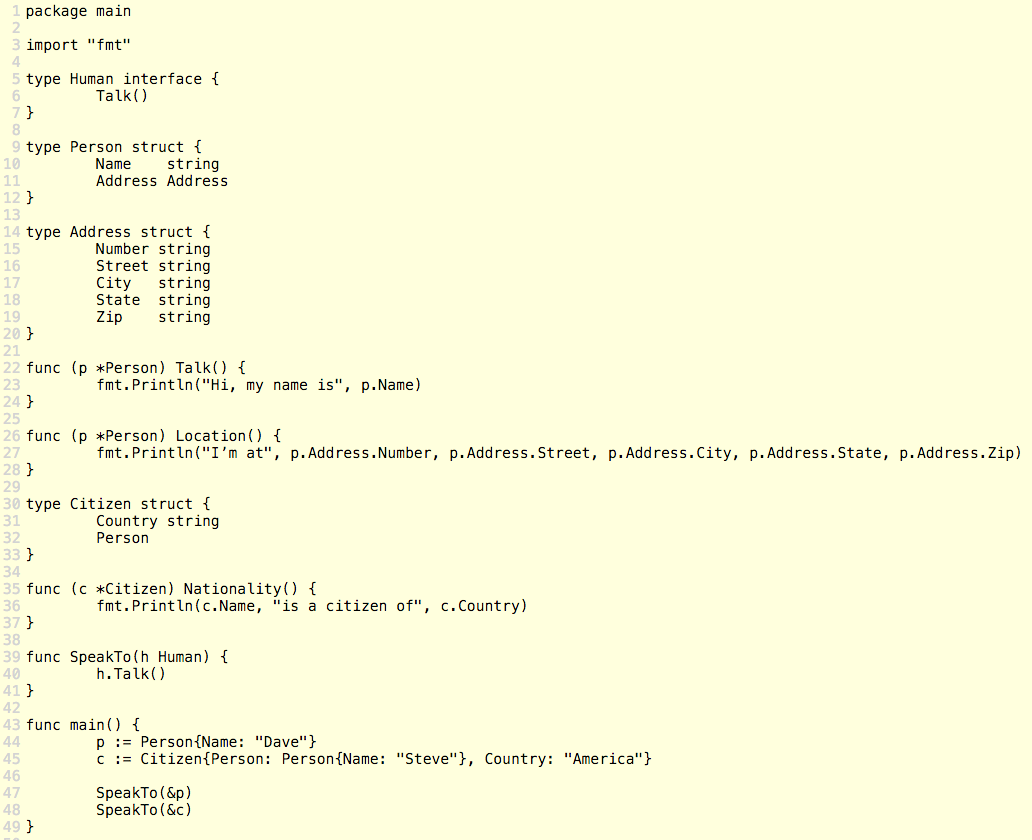
\includegraphics[width=0.7\linewidth]{interfacecode}
			\caption[Esempio di interfaccia]{Esempio di implementazione del true subtyping tramite interfaccia.}
			\label{fig:interfacecode}
		\end{figure}
	\end{frame}
	
	\begin{frame}
		\frametitle{True subtyping: interfaces}
		\begin{figure}
			\centering
			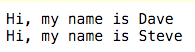
\includegraphics[width=0.7\linewidth]{interfaceresult}
			\caption[Esempio di interfaccia]{Risultato dell'esecuzione del codice precedente.}
			\label{fig:interfacecode}
		\end{figure}
	\end{frame}

	\begin{frame}
		\frametitle{Gestione degli errori?}
		\begin{itemize}[<+->]
			\item ...no!
			\item Go non implementa \textit{direttamente} meccanismi per gestire errori
			\item ogni funzione restituisce sempre un valore di errore insieme al risultato della sua computazione
			\item in base al valore di errore, il programmatore deve comportarsi di conseguenza
		\end{itemize}
	\end{frame}
	
	\begin{frame}
		\frametitle{Gestione degli errori?}
		\begin{figure}
			\centering
			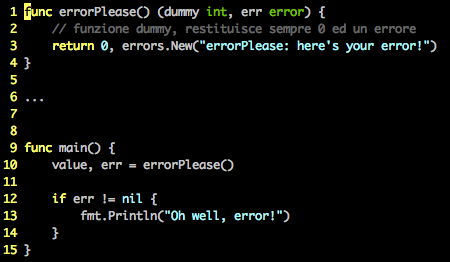
\includegraphics[width=0.7\linewidth]{funcerror}
			\caption[Errore]{Esempio di dichiarazione e gestione di funzione con valore di errore}
			\label{fig:funcerror}
		\end{figure}
	\end{frame}
	
	\begin{frame}
		\frametitle{Testing!}
		\begin{itemize}[<+->]
			\item Go include un sistema per testare il codice
			\item \textbf{Esempio:} il sorgente chiamato "Fle.go", viene testato da "Fle\_test.go"
			\item ogni pacchetto può essere testato dal comando \textit{go test}
		\end{itemize}
	\end{frame}
	
	\begin{frame}
		\frametitle{Testing!}
		\begin{figure}
			\centering
			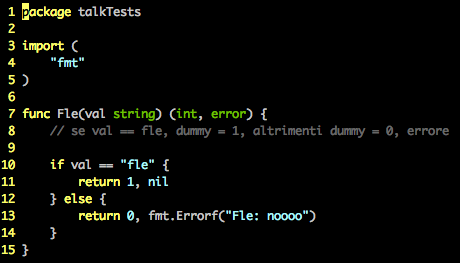
\includegraphics[width=0.7\linewidth]{testfunc}
			\caption[Funzione test]{Funzione da testare}
			\label{fig:testfunc}
		\end{figure}
	\end{frame}
	
	\begin{frame}
		\frametitle{Testing!}
		\begin{figure}
			\centering
			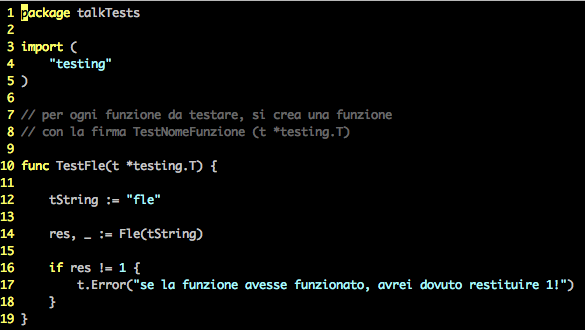
\includegraphics[width=0.7\linewidth]{realtestfunc}
			\caption[Funzione test]{Funzione di testing}
			\label{fig:testfunc}
		\end{figure}
	\end{frame}
	
	\begin{frame}
		\frametitle{Testing!}
		\begin{figure}
			\centering
			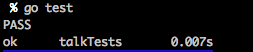
\includegraphics[width=0.7\linewidth]{result}
			\caption[Risultato]{Risultato del testing}
			\label{fig:testfunc}
		\end{figure}
	\end{frame}
	
	\begin{frame}
		\frametitle{Links}
		\begin{itemize}
			\item \url{http://play.golang.org/}
			\item \url{https://golang.org/}
			\item \url{https://tour.golang.org}
			\item \url{https://golang.org/doc/faq}
		\end{itemize}
	\end{frame}
\end{document}